\chapter{The dataset}\label{cha:data}

This chapter introduces the dataset and prepossessing steps taken to enable information extraction and analysis of the provided data. In addition it introduces how the case used in the analysis. 


% In the data set, there are three power plants that have pelton turbines with measurement of their needle position. More information about a pelton turbine can be found in chapter \ref{cha:data}. One of the power plants had recorded several issues with the control and behaviour of the needles during operation. There were many interesting events spread out over many of the power plants, but one major benefit with the pelton needle case, was that there was one plant with several reported issues for the same component. In most of the other cases, there were only recorded one incident on one plant, making them hard to analyze and validate. The fact that there also were two power plants in addition that had the same process signals without reported issues, opened up the possibility for testing and validating the chosen techniques not only on data from the faulty plant. This also introduced the possibility to validate how well and how easy the different techniques could adapt to new plants.    




% Based on the arguments above, the pelton needle case was chosen as the focus of the thesis. The following points were then defined as a basis for the analysis. 


\section{Dataset}\label{sec:dataset}
    Hymatek controls provided a dataset from a Norwegian energy company, containing process information from $27$ hydro electric powerplants logged from $2013$ to mid $2017$. The data was not pre-prosessed in any way, and came just as it had been logged at the company. A big part of the thesis has been spent on exploring the data, finding out what is logged and what can be used. The data was split into five folders, one for each year. In each folder several different files were stored. Table \ref{tab:data_files} shows the different file types that were found in the dataset. The file names indicated the frequency, sampling type and sampling duration of the data. The files were not separated by plants, only by date. Hence, a file containing data sampled every second for any given start and stop date, would contain all secondly sampled data from all plants for that given period. In addition to the datafiles, a meta-data file was provided where plant name and process signal for each tag could be found. \cite{}
    
    \begin{table}[]
        \centering
        \begin{tabular}{|c|c|c|c|c|}
            \hline
             Interval   & Average   & Max   & Min   & Actual    \\ \hline
             Daily      & x         & x     & x     & -         \\ \hline
             Hourly     & x         & x     & x     & -         \\ \hline
             Minutely   & x         & x     & x     & -         \\ \hline
             Secondly   & -         & -     & -     & x         \\ \hline
        \end{tabular}
        \label{tab:data_files}
        \caption{Table showing the available data for the different sampling frequencies}
    \end{table}
    
    The total size of all files exceeded $90$Gb, this meant that one could not simply just read all data into the ram and work with it from there. The information needed to be extracted for one plant at a time, for each of the different sampling rates, and stored in a way that enabled fast and efficient loading. All of the work with reading, processing and storing the data was done in python using the \textbf{Pandas} library. The \textbf{Pandas} package \cite{Mckinney2010} provides efficient and intuitive methods and data structures that serves as a great basis for data analysis. 
    
    
    
    \subsection{Old and new data format}\label{subsec:data_format}
        Regardless of sampling-rate and data type, the files were all on the same format. As seen in table \ref{tab:orig_data}, each line held a tag, a time of sampling and a process value. 
        
        \begin{table}[h]
            \centering
            \begin{tabular}{|c c c|}
                \hline
                 Tag        & Timestamp         & Value  \\
                 192390514  & 20170101000000000 & 0.897244155 \\
                 192391514  & 20170101000000000 & -0.549806237 \\
                 \hline
            \end{tabular}
            \caption{Example of the structure of the original datasets}
            \label{tab:orig_data}
        \end{table}
        
        Once a file was loaded the tag was replaced by the process-signal name found in the meta-data file. To enable interpretation and analysis of the data, it was decided that new datasets needed to be created. The format shown in table \ref{tab:plant_format} was chosen. When all samples from a given plant were extracted, and the tag replaced by the process name, the data matrix were reconstructed to hold the format shown in table \ref{tab:plant_format}
        
        \begin{table}[h]
            \centering
            \begin{tabular}{|c|c|c|c|c|}
                \hline
                Time stamp & P. variable 1     & P. variable 2    & ..    & P. variable n    \\ \hline
                time 1        & NaN         & $2$           & ..    & NaN         \\ \hline
                time 2        & $3.00$      & NaN           & ..    & $0.00214$\\ \hline
            \end{tabular}
            \caption{Example showing how the data could look in the data format for each plant after reconstruction is complete}
            \label{tab:plant_format}
        \end{table}

        
    \subsection{Overview of the datasets}
        Once the data was reconstructed as specified in subsection \ref{subsec:data_format} one could look into what information they held. The number of available process signals varied a lot, from above $250$ to below $20$, as can be seen in figure \ref{fig:process_signal_overview}. This was used as a first stage filtering to reduce the number of plants to examine. The plants with fewer than $30$ process-signals were dropped from the analysis, reducing the number of plants in the dataset to $15$.    
        
        \begin{figure}[h]
            \centering
            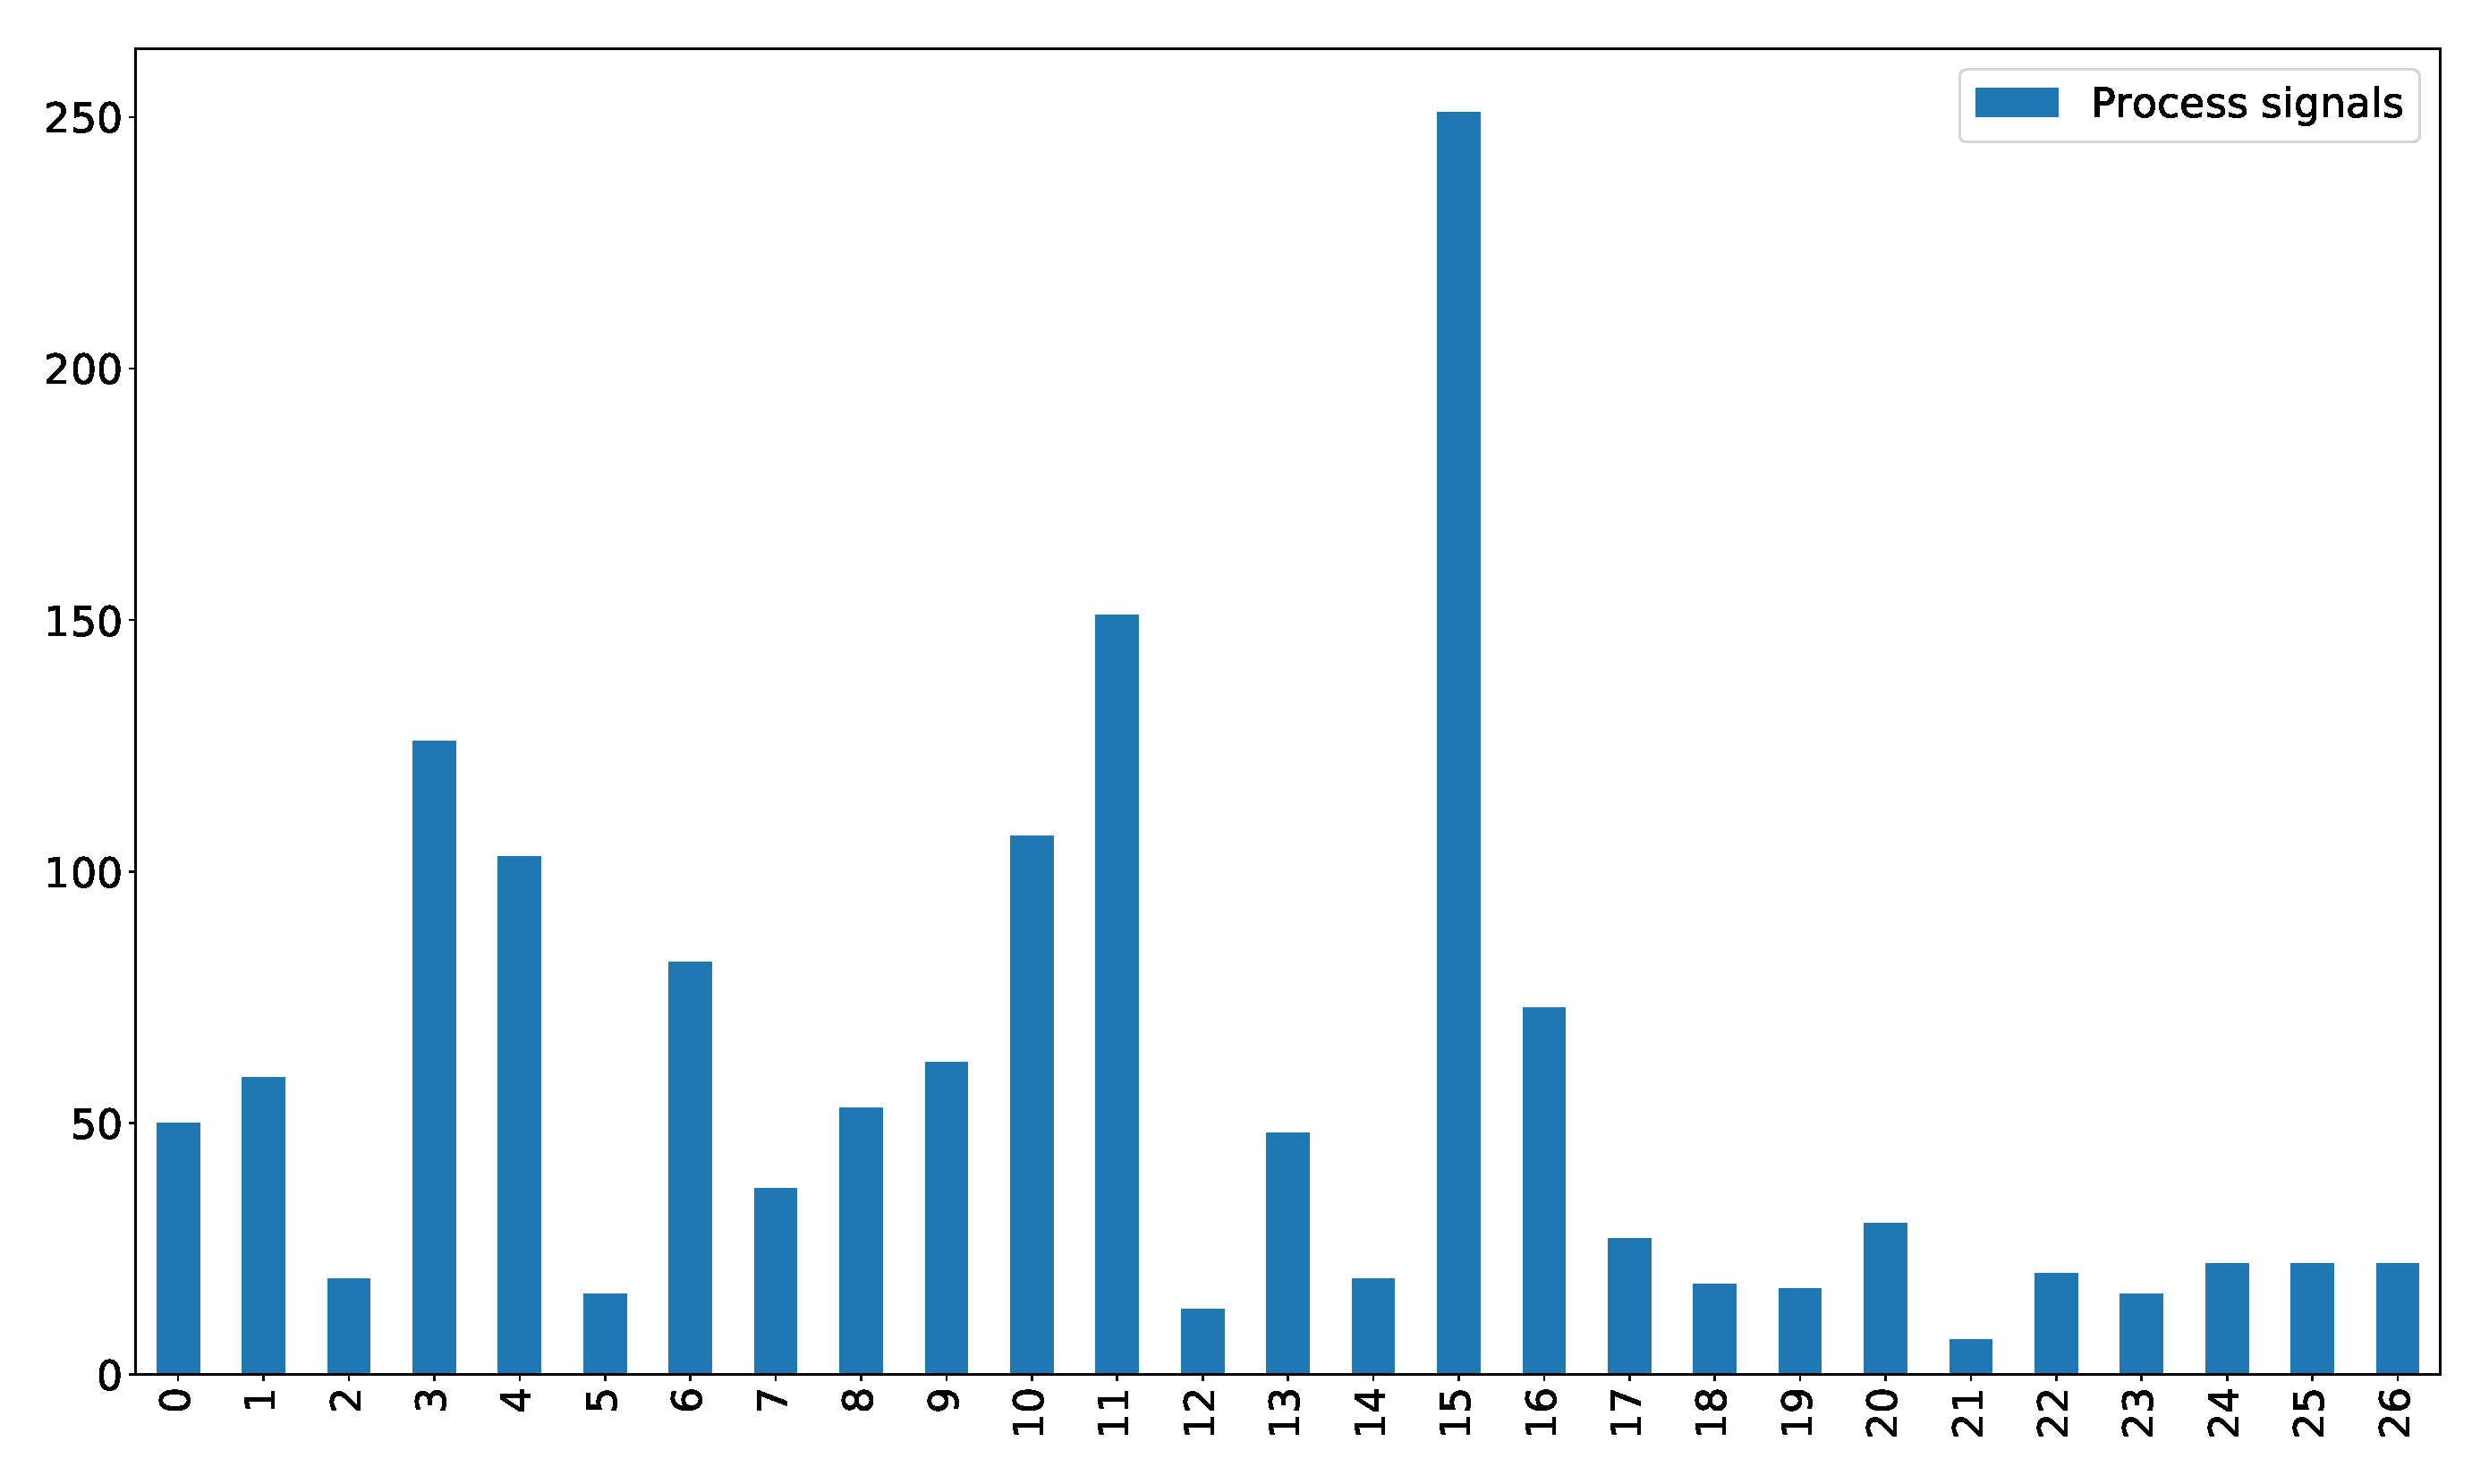
\includegraphics[width=\textwidth]{report/figures/data/plant_process_signals_overview.pdf}
            \caption{Overview of the number of process-signals for each of the 27 plants}
            \label{fig:process_signal_overview}
        \end{figure}
        
        After discarding the plants with few signals, the type of process-signals available were looked into. The more data sampled from different parts of a plant, the better. Having data from several parts and components of a plant can enable finding a link between unknown components and sensors. This can then be used to improve the knowledge of a plant beyond the pure measurements taken by each sensor. Figure \ref{fig:signal_type_overview} shows the different types of signals found in the datasets for the different plants. As can be seen temperature is one of the most common signals for all plants. There is also many signals of type "Def Type Måling", which is a common name that covers all signals not defined. Pressure, level, vibration, etc are signals covered by this tag. Since all of the remaining plants had process-variables of different types, none were removed. 
        
        \begin{figure}
            \centering
            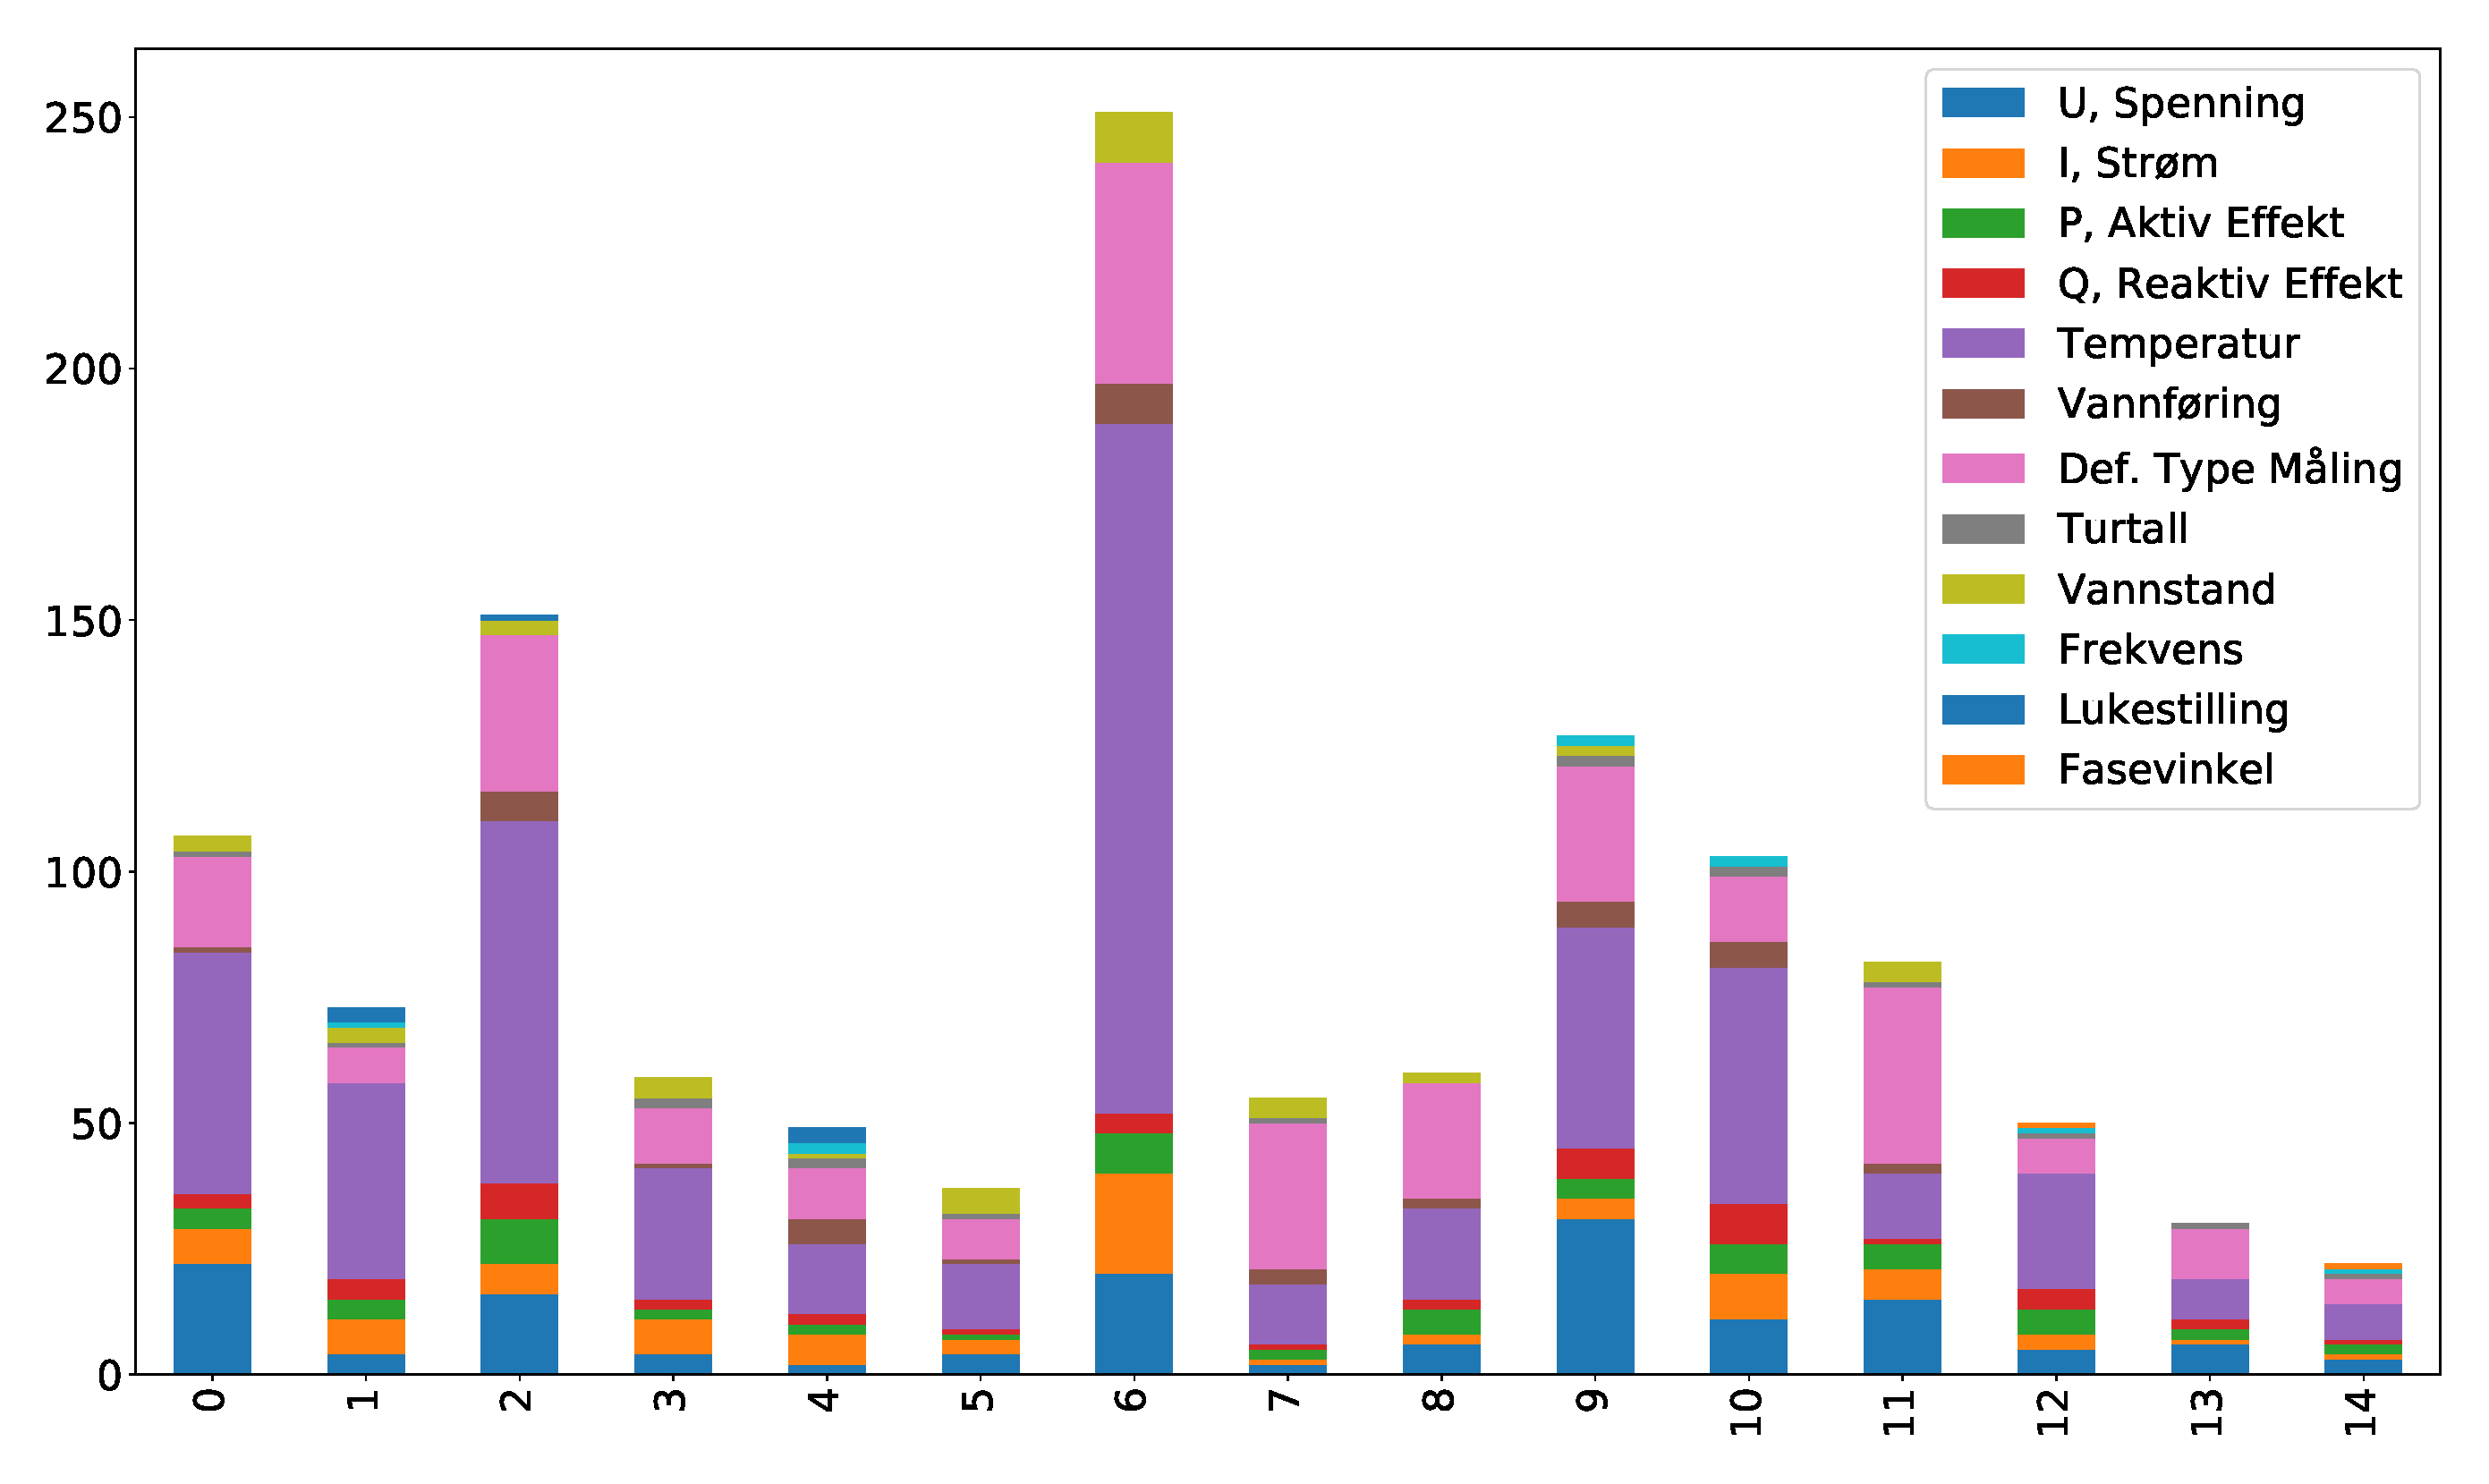
\includegraphics[width=\textwidth]{report/figures/data/plant_signal_types_overview.pdf}
            \caption{Figure showing the different variables found and the number of them in each plant dataset}
            \label{fig:signal_type_overview}
        \end{figure}
        
        % It is only necessary to keep the datasets with the highest sampling rate. The highest sampling rate will provide the most detail about a plant, and lower sampling rates can always be extracted from higher rates.
        
        % was decided to only use the datasets sampled every second. Using these datasets gave a snapshot of the plant state at a given time. Pandas has a lot of built in functionality that enables easy re-sampling, so that the average, max and min datasets could easily be recreated from this dataset if wanted.
        
        An issue arose when looking in detail at the datasets. Preferably, all process-signals should be sampled periodically and at the same time. This was however not the case, only at hourly resolution where the data matrices complete. At higher sampling rates there were a lot of missing data. At the highest sampling frequency (every second), there were many time-stamps were none of the process signals were sampled, and those that were sampled often only sampled one process-signal. This meant that one either had to work with only hourly sample rate, work with incomplete datasets or use some sort of missing data technique to fill the gaps in the datasets. Either the equipment used for sampling is not working as it should, or the varying sampling rate must be done on purpose. One can however, not find any reason for using such a sample scheme. This sheds light on the fact that having lots of data is not always a sign of quality. This issue will be further discussed in the analysis. It was found that the data sampled in $2013$ was poorer than the later years, and hence it was dropped from any further analysis. 
    % \subsection{Instrumentation}\label{subsec:instrumentation}
    %     what is there of instrumentation? refer to the data I have gotten         
        
    \subsection{The historical log of the plants }
        Once an overview of the data was in place, the energy company was contacted, requesting an incident log from the remaining plants. Logs for all of the $27$ power plants were received, holding information about small to large incidents that had occurred during the sampling period. The level of details in the logged incidents were very varying from plant to plant. Some plants had reported over 200 incidents, while other barely exceeded 20. Many of the incidents were also minor incidents like a broken light bulb or non functioning tools. This made the work for finding interesting incidents time consuming. There were found several interesting incidents, but very few were reported to occur more than once. Having few incidents makes it hard to separate valuable information from noise. Only having a limited number of faults can easily lead to overfitting. There is always a risk that the correlations and variable dependencies found can be caused by randomness. If one don't have enough erroneous observations to ensure that one is not modeling randomness and noise, the results can end up looking great, when in reality the solution is worthless on new data. 
        
        The energy company reported an error with the needles of a Pelton turbine from one of the plants. As the power production decreases below $46\%$ one needle was reported to lag behind a needle it was operated with. This given plant has two Pelton turbines, with the same setup. \todo{what was done to fix this? what was the problem exactly? why was it not discovered?} These turbines have four needles each. When looking into the historical log of the plant, it was found that several more incidents with the Pelton needles were reported for the two turbines. A search through the $14$ remaining power plants, showed that there were two additional plants with Pelton turbines. One with four needles and one with five. These plants had however not reported any problems with the Pelton needles. This meant that one could assume to have data without error, which could be used as reference. It is also beneficial that techniques can be tested on different datasets, it can then be confirmed whether or not the techniques can be used without any alteration on new data, and what needs to be done before they can. 
        
        
        
\section{Pelton needles case}\label{sub:pelton_needles}
    The Pelton needle case was chosen for further analysis for several reasons. Firstly it is a critical part of the Pelton turbine, if the needles are not operating as they should it will affect the power produced by the turbine. The needle openings are a big part of a complex control-system, and controls that the turbine holds constant speed. If a method can be found that could give early warnings about the above mentioned incident, maintenance can be planned and components can be overhauled before the system condition becomes so bad that it is no longer controllable. Secondly, having data from different plants makes it possible to analyze how well the methods and techniques used adapt to new data. This is an important factor, if one can develop a method that is transferable with little to no adaptation need between plants, the time for commissioning will be greatly reduced. In addition, this case fits well as a extension of my project thesis, where the condition of the guide vanes for a Francis turbine was analyzed. Finally, quality and available process variables varied a lot from plant to plant. One of the biggest issues was that the majority of the process signals were not sampled at a constant frequency. Often only one process-signal were logged for each time stamp giving a data matrix not straight forward to analyze. For the Pelton needle case, sample frequency and simultaneous sampling of several process signals were among the best in the dataset.
             

    \subsection{Incident 02.03.2017}
        As the incident reported that one needle was lagging behind another, it could mean that they were pairwise operated. To investigate how the needles were operated with regards to one another, scatter-plots were created where each needle was plotted against the other. To enable this the needle process signals were pairwise extracted from the rest of the dataset, and all time-stamps where both needles were not sampled were removed. This meant that each time-stamp must be considered as a snapshot of the plant, and trends from one time-step to another not could be interpreted easily. 
        
        % The left figure in figure \ref{fig:pairwise_needles} shows an example of two needles that are pairwise operated. The opening of the needles are following each other linearly. The right figure show two needles that are not pairwise operated, at higher openings the needles seems to follow one another, but at lower openings this is not the case. This is because a Pelton turbine controls its power output by varying the number of active needles. Hence at full power all needles will be operated similarly, but at lower power some of the needles will not be operated. This is seen by all the samples found at zero opening for needle four, but at higher opening for needle three. 
        
         Figure \ref{fig:plant1_needles} shows the scatter-plot of the pairwise operated needles for plant 1. As can be seen by the dark blue area, all four plots have a linear dependency between the needles. However, there is clearly several data-points that deviate from this, especially for needle pair $[2,4]$ on turbine $2$. The reported error occurred on turbine #$2$ with needle $4$ lagging behind needle #$2$. The plot in the bottom right corner clearly shows that there are several samples where the two needles are operating incorrectly. There are also tendencies to problems with needle #$1$ and needle #$3$ for the same turbine. Turbine $1$ is doing better, but for needle #$2$ and #$4$ there are some samples that are not as they should. 
        
        \begin{figure}[h]
            \centering
            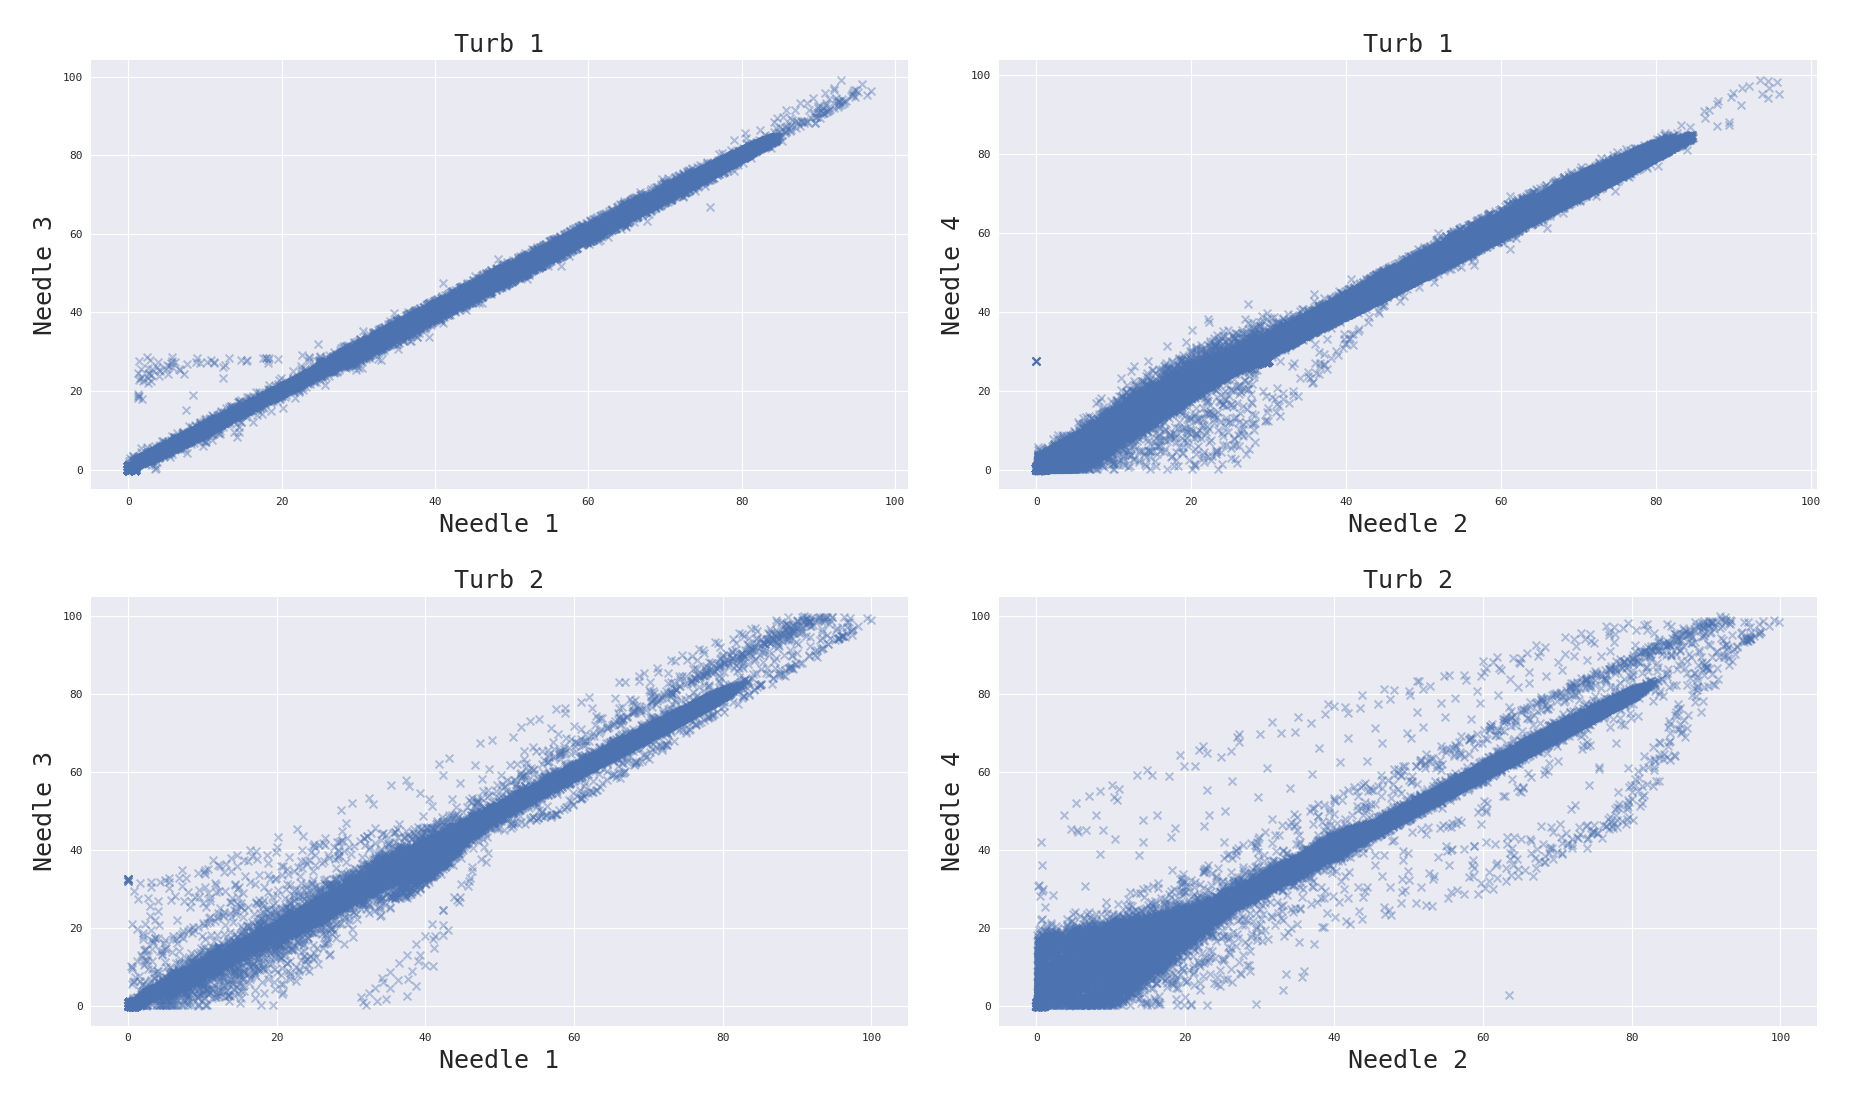
\includegraphics[width=\textwidth]{report/figures/data/plant1_needles.png}
            \caption{Pairwise operated needles for plant 1}
            \label{fig:plant1_needles}
        \end{figure}
        
        Figure \ref{fig:n_pos_2802} to \ref{fig:n_pos_aft_0303} shows the needle positions for the dates surrounding the reported incident. As can be seen in figure \ref{fig:n_pos_aft_0303}, the issue with the needles is fixed and they behave as intended. Figure \ref{fig:n_pos_0203} and \ref{fig:n_pos_0303} shows the two days with worst performance, and one can see that many of the worst data-points from the lower right plot in figure \ref{fig:plant1_needles} looks to be the same as the ones shown in figure \ref{fig:n_pos_0203} and \ref{fig:n_pos_0303}. There are also outliers in figure \ref{fig:n_pos_0103} and \ref{fig:n_pos_2802}, this gave rise to the idea that it might be possible to detect the degradation of the system behaviour before it becomes to critical, using the data after the incident to represent normal system operation.
        \begin{figure}[h]
            \caption*{Turbine 2 needle positions}
            \begin{minipage}[b]{0.5\linewidth}
                \centering
                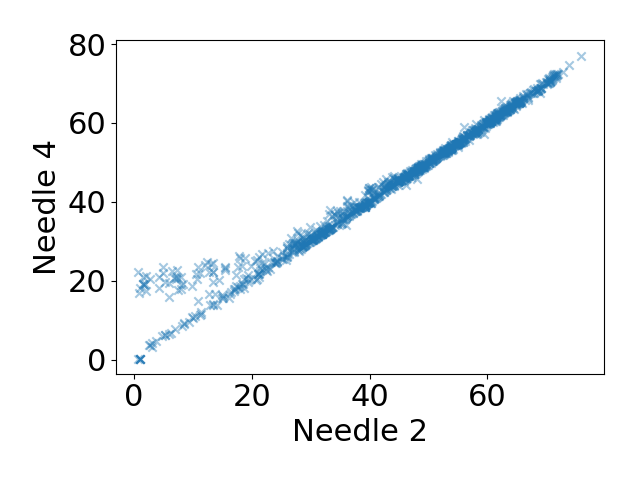
\includegraphics[width = \textwidth]{report/figures/data/turb2_n2_n4_28022017.png}
                \caption{28.02.2017}
                \label{fig:n_pos_2802}
            \end{minipage}
            \begin{minipage}[b]{0.5\linewidth}
                \centering
                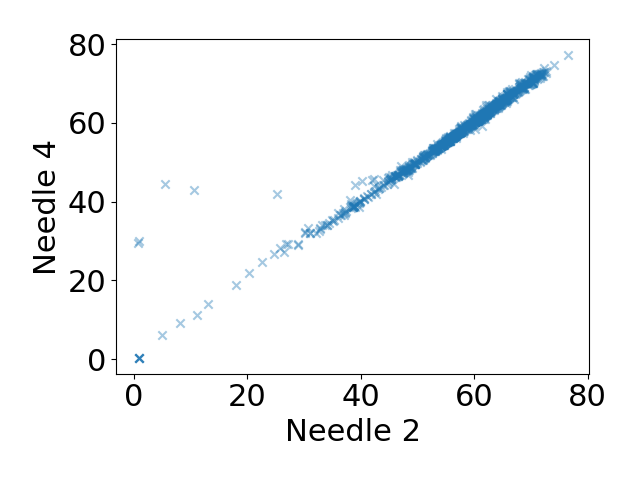
\includegraphics[width = \textwidth]{report/figures/data/turb2_n2_n4_01032017.png}
                \caption{01.03.2017}
                \label{fig:n_pos_0103}
            \end{minipage}
            \begin{minipage}[b]{0.5\linewidth}
                \centering
                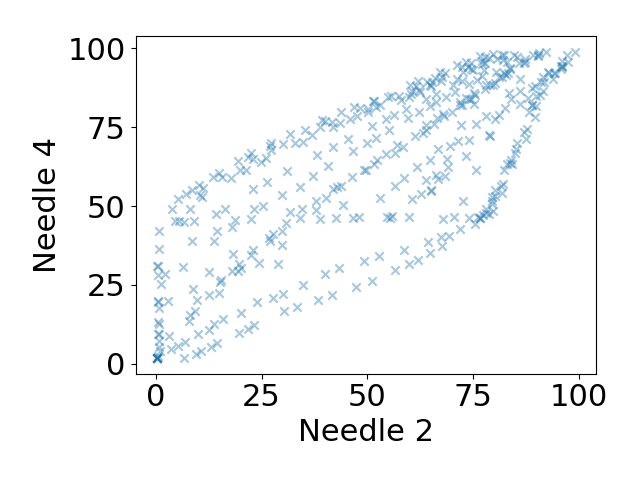
\includegraphics[width = \textwidth]{report/figures/data/turb2_n2_n4_02032017.png}
                \caption{02.03.2017}
                \label{fig:n_pos_0203}
            \end{minipage}
            \begin{minipage}[b]{0.5\linewidth}
                \centering
                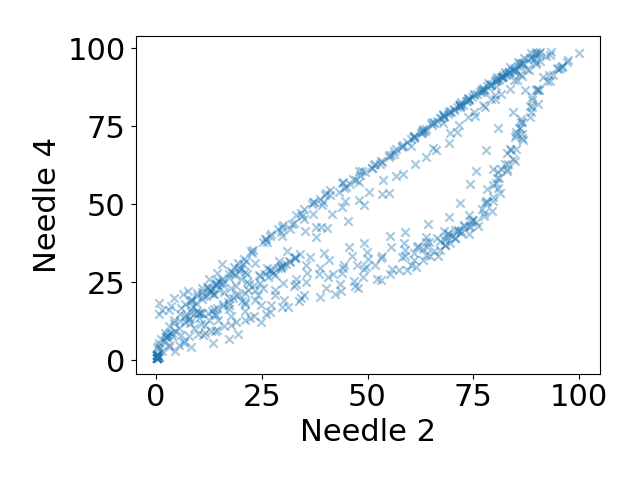
\includegraphics[width = \textwidth]{report/figures/data/turb2_n2_n4_03032017.png}
                \caption{03.03.2017}
                \label{fig:n_pos_0303}
            \end{minipage}
            \begin{minipage}[b]{0.5\linewidth}
                \centering
                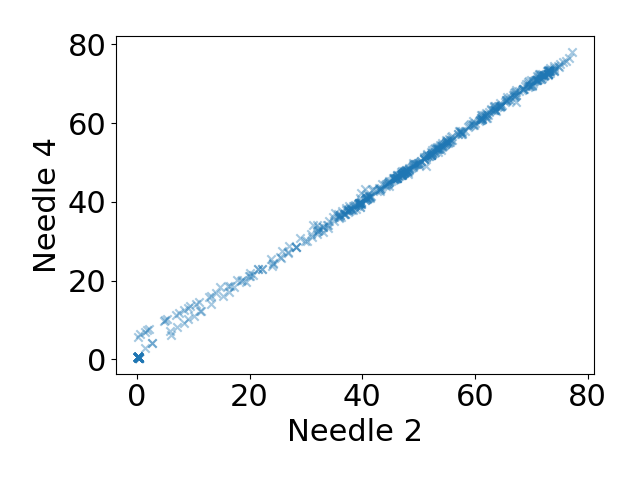
\includegraphics[width = \textwidth]{report/figures/data/turb2_n2_n4_after_04032017.png}
                \caption{04.03.2017 ->}
                \label{fig:n_pos_aft_0303}
            \end{minipage}
        \end{figure}
        
        To further analyze if the Pelton needle case could be used, the needle position and the difference between them were plotted as seen in figure \ref{fig:plant1_needle_error}. The reported incident $02.03.2017$ can clearly be seen in the plot. Both the error and the RMSE between the two needles are much lower after the incident than before. It can also look like the error steadily grows from $01.10.2016$. It also looks like there has been issues with the needle pair at earlier occasions to. There is a spike in $2014$ and some some issues in early $2016$. However, there is not reported any issues with either needle two or four in those periods. But the error is also smaller than it was during the incident 02.03.2017, so it might not be enough to catch their attention. 
        
        \begin{figure}
            \centering
            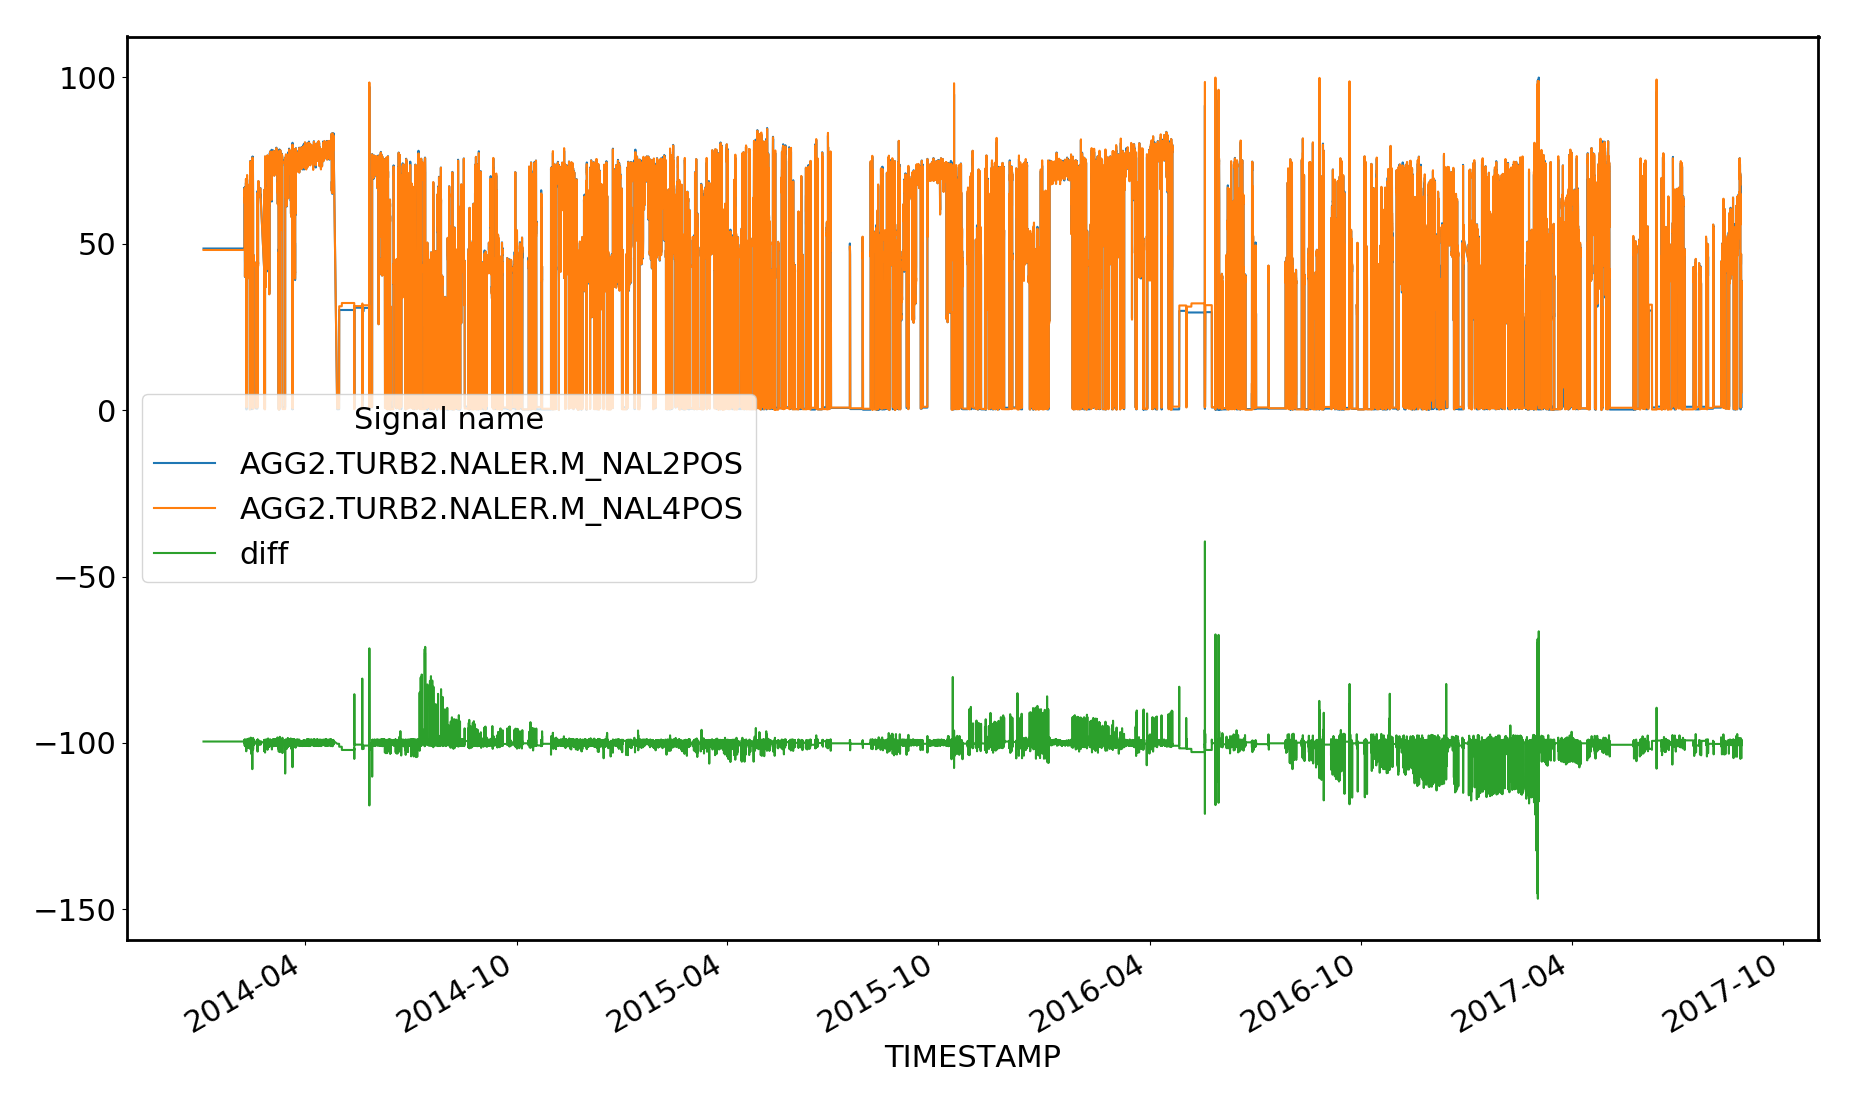
\includegraphics[width=\textwidth]{report/figures/data/turbine2_needle2_4.png}
            \caption{Overview of needle error for turbine 2, needle [2,4] on plan 1}
            \label{fig:plant1_needle_error}
        \end{figure}
        
        
    \subsection{Other incidents}
        The log reported two other needles issues with plant $1$ that are possible to track with the needle scatter plots they can be seen in figure \ref{fig:start_failure_turb1} and \ref{fig:start_failure_turb2}. Both are start up failures due to problems with the needle operation. The failure on 10.12.2014 has a similar pattern as the reported incident, and can then be used as a test case.
        \begin{figure}[h!]
            \caption*{Start up errors}
            \begin{minipage}[b]{0.5\linewidth}
                \centering
                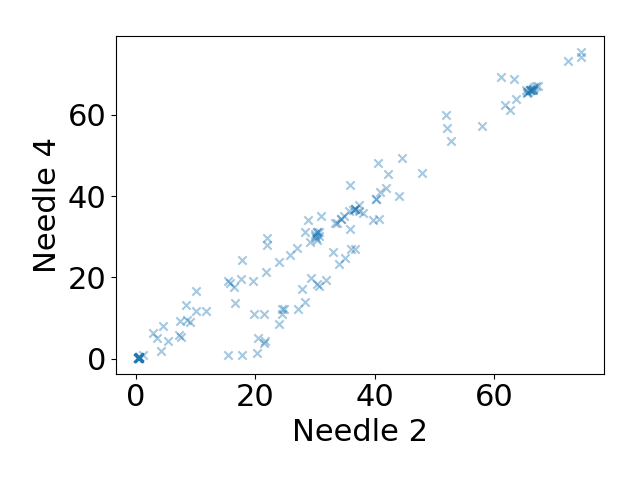
\includegraphics[width = \textwidth]{report/figures/data/turb1_n2_n4_scatter_start_failure_10122014.png}
                \caption{Turbine 1, 10.12.2014}
                \label{fig:start_failure_turb1}
            \end{minipage}
            \begin{minipage}[b]{0.5\linewidth}
                \centering
                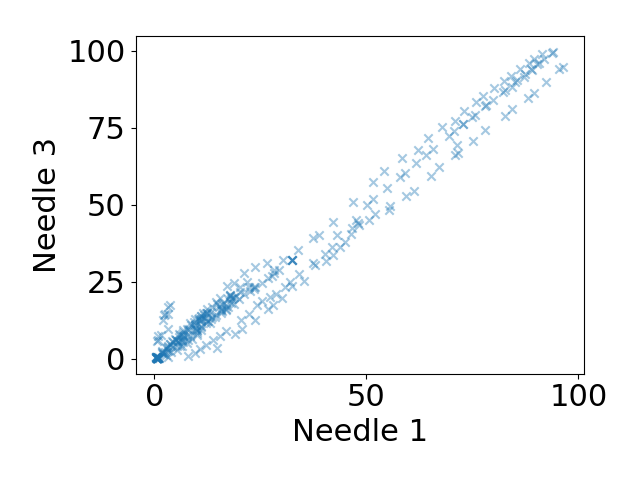
\includegraphics[width = \textwidth]{report/figures/data/turb2_n1_n3_start_failure_25082016.png}
                \caption{Turbine 2, 25.08.2016}
                \label{fig:start_failure_turb2}
            \end{minipage}
        \end{figure}
        
        
    
    \subsection{Other plants}
        Further investigation showed that in addition to the plant that reported the incident, one of the other plants with Pelton turbines also had two turbines with pairwise operated needles. This meant that there were data available from four different turbines, that could be used for analysis. The third plant only had one Pelton turbine, and here the needles were not pairwise operated. The turbine used from 1 to 5 needles depending on the the produced power, and which needles were operated were rotated, most likely so that all needles should have the same amount of wear. Extracting periods where two or more needles are operated similarly could be used to extend the analysis.   
        
        For plant #$2$ one can see in figure \ref{fig:plant2_needles} that turbine #$1$ has no sampling on needle #$1$, this means that this plant has three useful datasets. Based on plant 2 it becomes clear that there is something wrong with the needles for plant $1$. All needle pairs follow the linear pattern much better, and have very few outliers. This data can then be used for cheking if the algorithms wrongly detects outliers.
        
        \begin{figure}
            \centering
            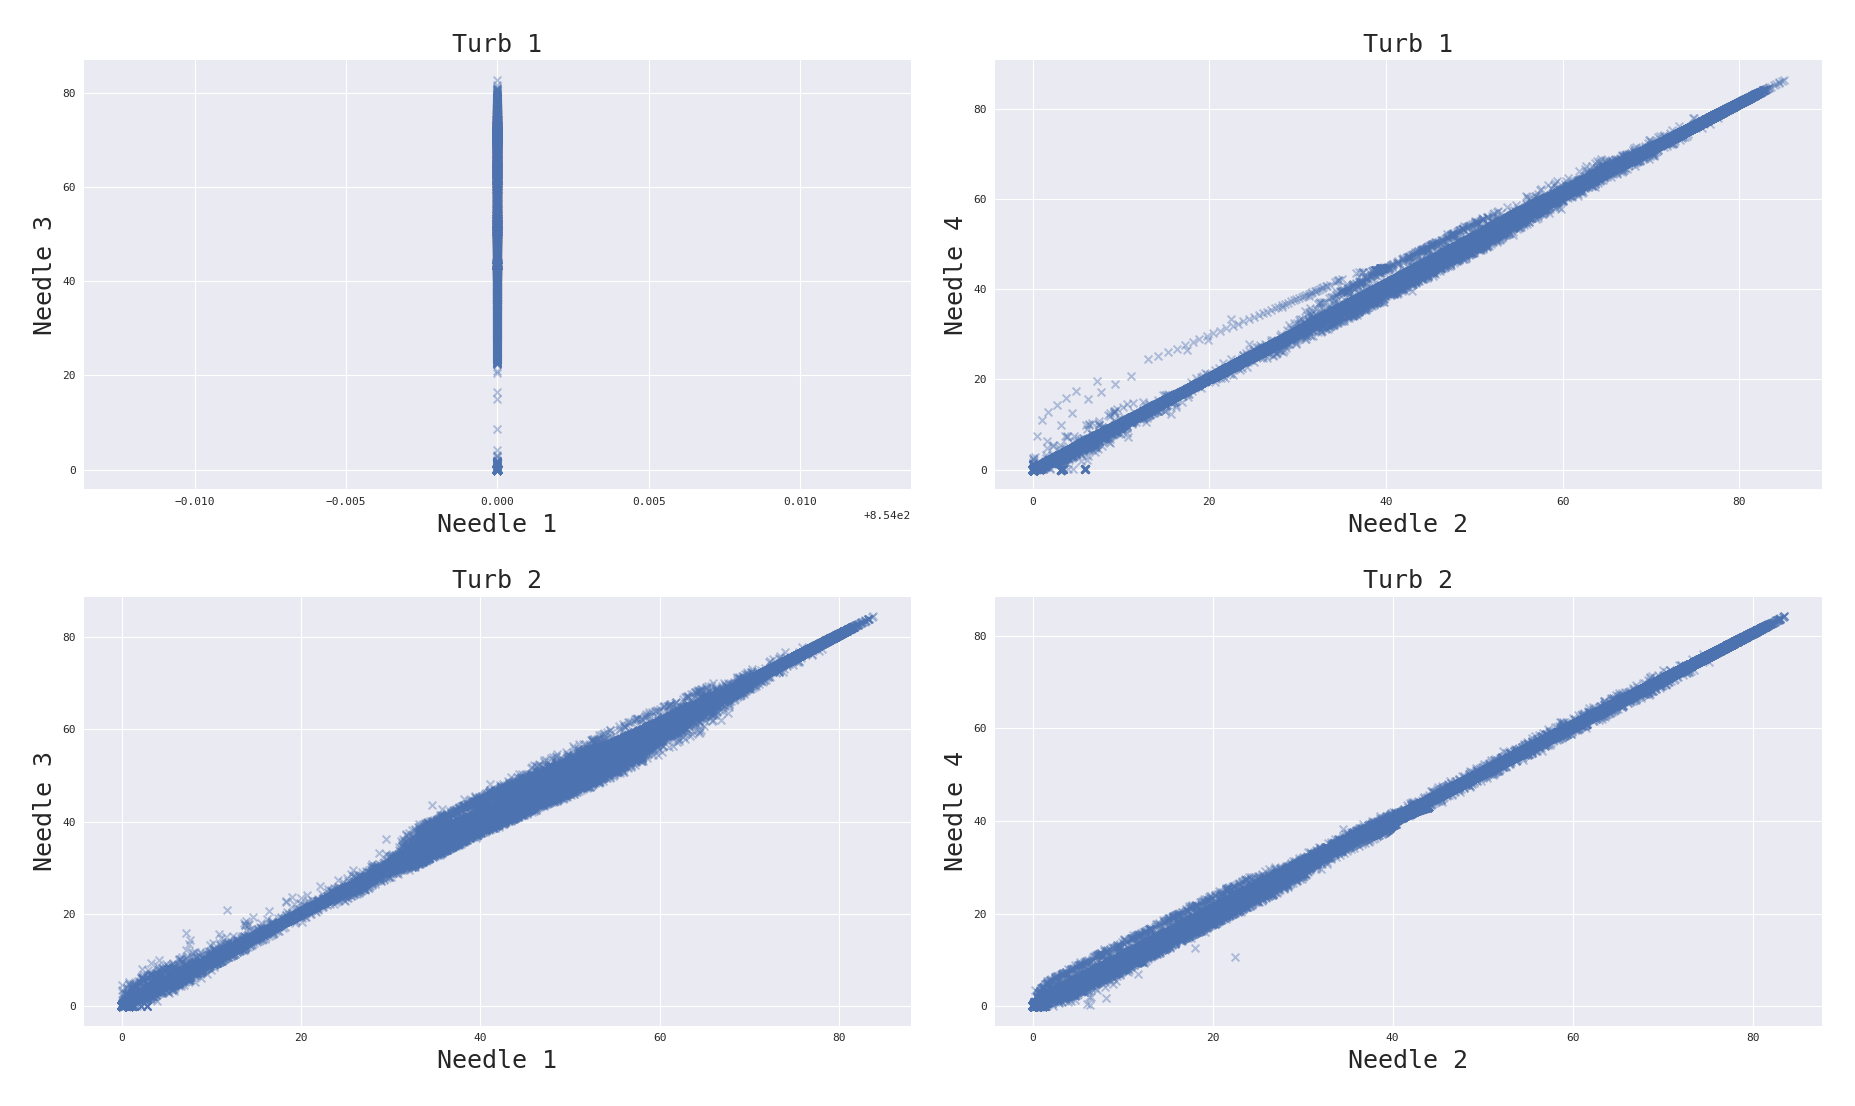
\includegraphics[width=\textwidth]{report/figures/data/plant_2_needle_plot.png}
            \caption{Pairwise operated needles for plant 2}
            \label{fig:plant2_needles}
        \end{figure}
        
        
        
    % \section{Other process signals}
        
    
        
    %     mention that this alone is a case one can build upon but to track the error to other processvariable would be very interesintg both for condition monitoring but also for identification of the fault and why it happened. 
        
        
    %     It is important to understand that an outlier in the data does not necessarily mean that something is about to break. There is a possibility that the sample is an indication of a condition change in the equipmnet, but it might also be due to error in the measurement, noise or just a deviation in the ongoing process. This makes this kind of analysis even harder, an outlier might just be a coincident, that yields little to no information. 
        
         
         
        